\section{Data and Results}

\begin{figure}[h]
        \begin{subfigure}{0.5\textwidth}
                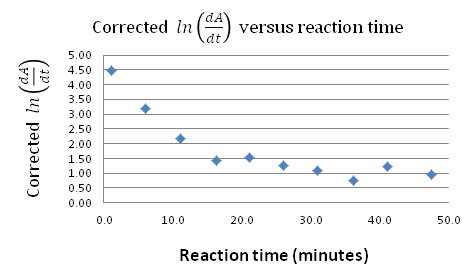
\includegraphics[width=\textwidth]{./Figures/20M_dipic_readings.png}
                \caption{0.20 M dipic}
                \label{fig:0.20M_dipic_readings}
        \end{subfigure}\begin{subfigure}{0.5\textwidth}
                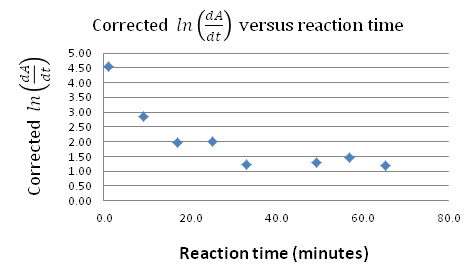
\includegraphics[width=\textwidth]{./Figures/10M_dipic_readings.png}
                \caption{0.10 M dipic}
                \label{fig:0.10M_dipic_readings}
        \end{subfigure}
        \begin{subfigure}{0.5\textwidth}
                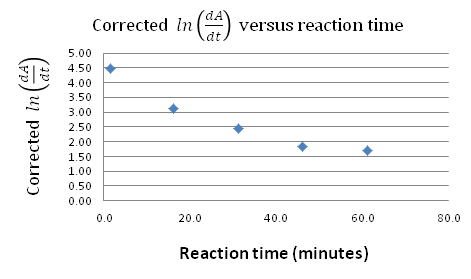
\includegraphics[width=\textwidth]{./Figures/05M_dipic_readings.png}
                \caption{0.05 M dipic}
                \label{fig:0.05M_dipic_readings}
        \end{subfigure}\begin{subfigure}{0.5\textwidth}
                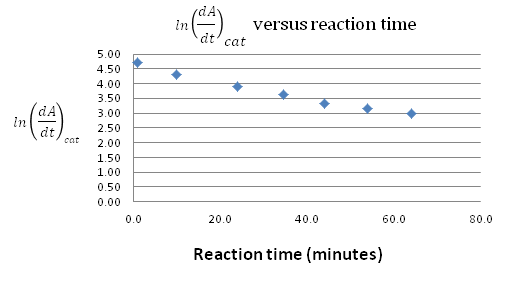
\includegraphics[width=\textwidth]{./Figures/016M_dipic_readings.png}
                \caption{0.016 M dipic}
                \label{fig:0.016M_dipic_readings}
        \end{subfigure}
        \begin{subfigure}{0.5\textwidth}
                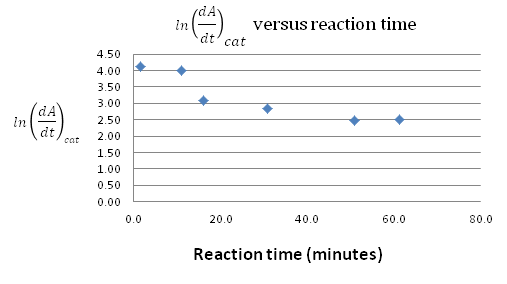
\includegraphics[width=\textwidth]{./Figures/032M_dipic_readings.png}
                \caption{0.032 M dipic}
                \label{fig:0.032M_dipic_readings}
        \end{subfigure}
        \caption{$ln \left(\frac{dA}{dt}\right)_{cat}$ measurements versus CA/dipic reaction time for various concentrations of dipic}\label{fig:start_times}
\end{figure}

\begin{table}[h]
    \begin{tabular}{| l | l | l |}
    \hline
    Constant & Empirical Value & Accepted Value \\ \hline
    $K_{EML}$ & $(20\pm{18}){\ }M^{-1}$ & foobar \\ \hline
    $k_{d}$ & $(0.10\pm{0.10}){\ }mins^{-1}$ & blah \\ 
    \hline
    \end{tabular}
    \caption[Table caption text]{Values of $K_{EML}$ and $k_d$, as determined in this experiment as well as accepted values from literature}
    \label{tbl:summary}
\end{table}